\newpage
\section{製作過程}
1.首先繪製球框。\
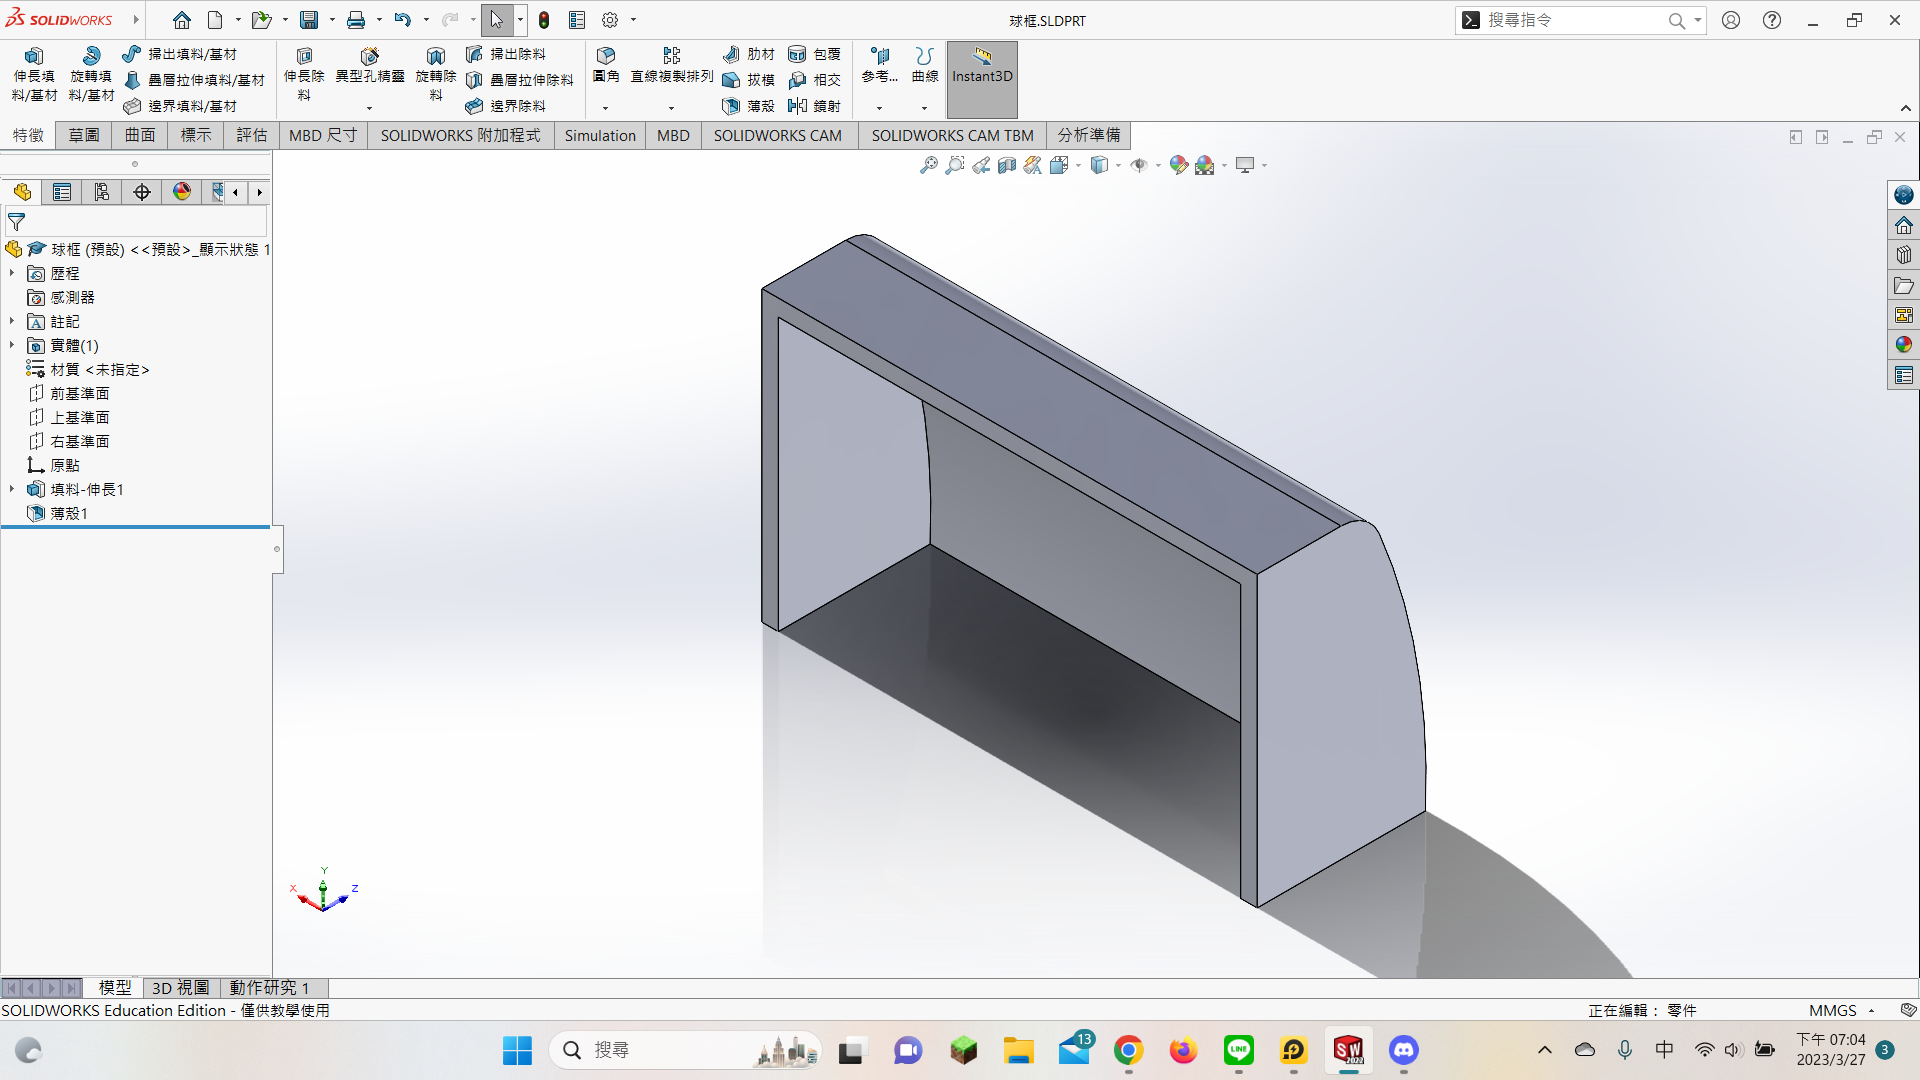
\includegraphics[angle=0,width=10cm]{2023-03-27}\\
\\2.這是lua腳本控制是bubbleRob前後左右sim.getObjectHandle這個函式在coppeliasim4.3.0版本被淘汰了但還是可以使用,但用sim.getObject會比較好在後面感測器腳本已做改善,這個程式是用上下左右控制bubbleRob空白鍵暫停開始。\
\begin{center}
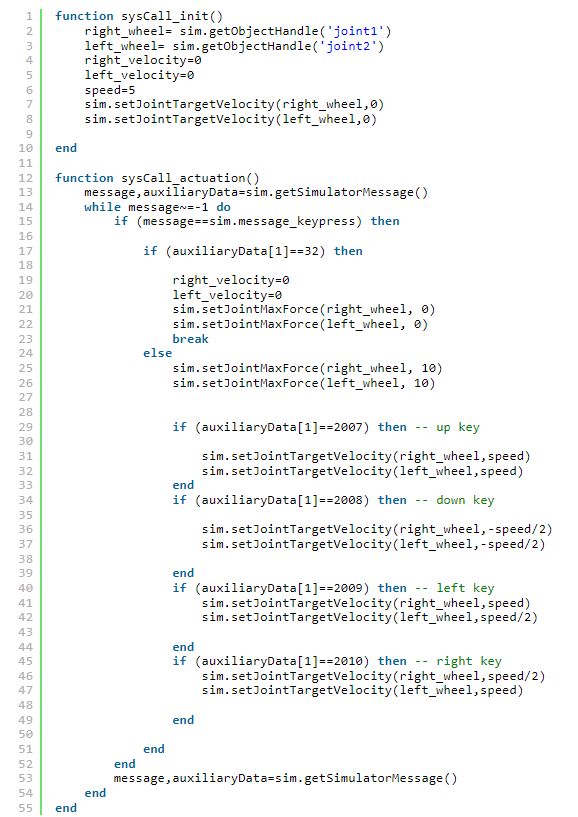
\includegraphics[angle=0,width=9cm]{螢幕擷取畫面 2023-04-14 221556}\\
\end{center}
 \newpage
3.加入球框感測器和記分板。\
\begin{center}
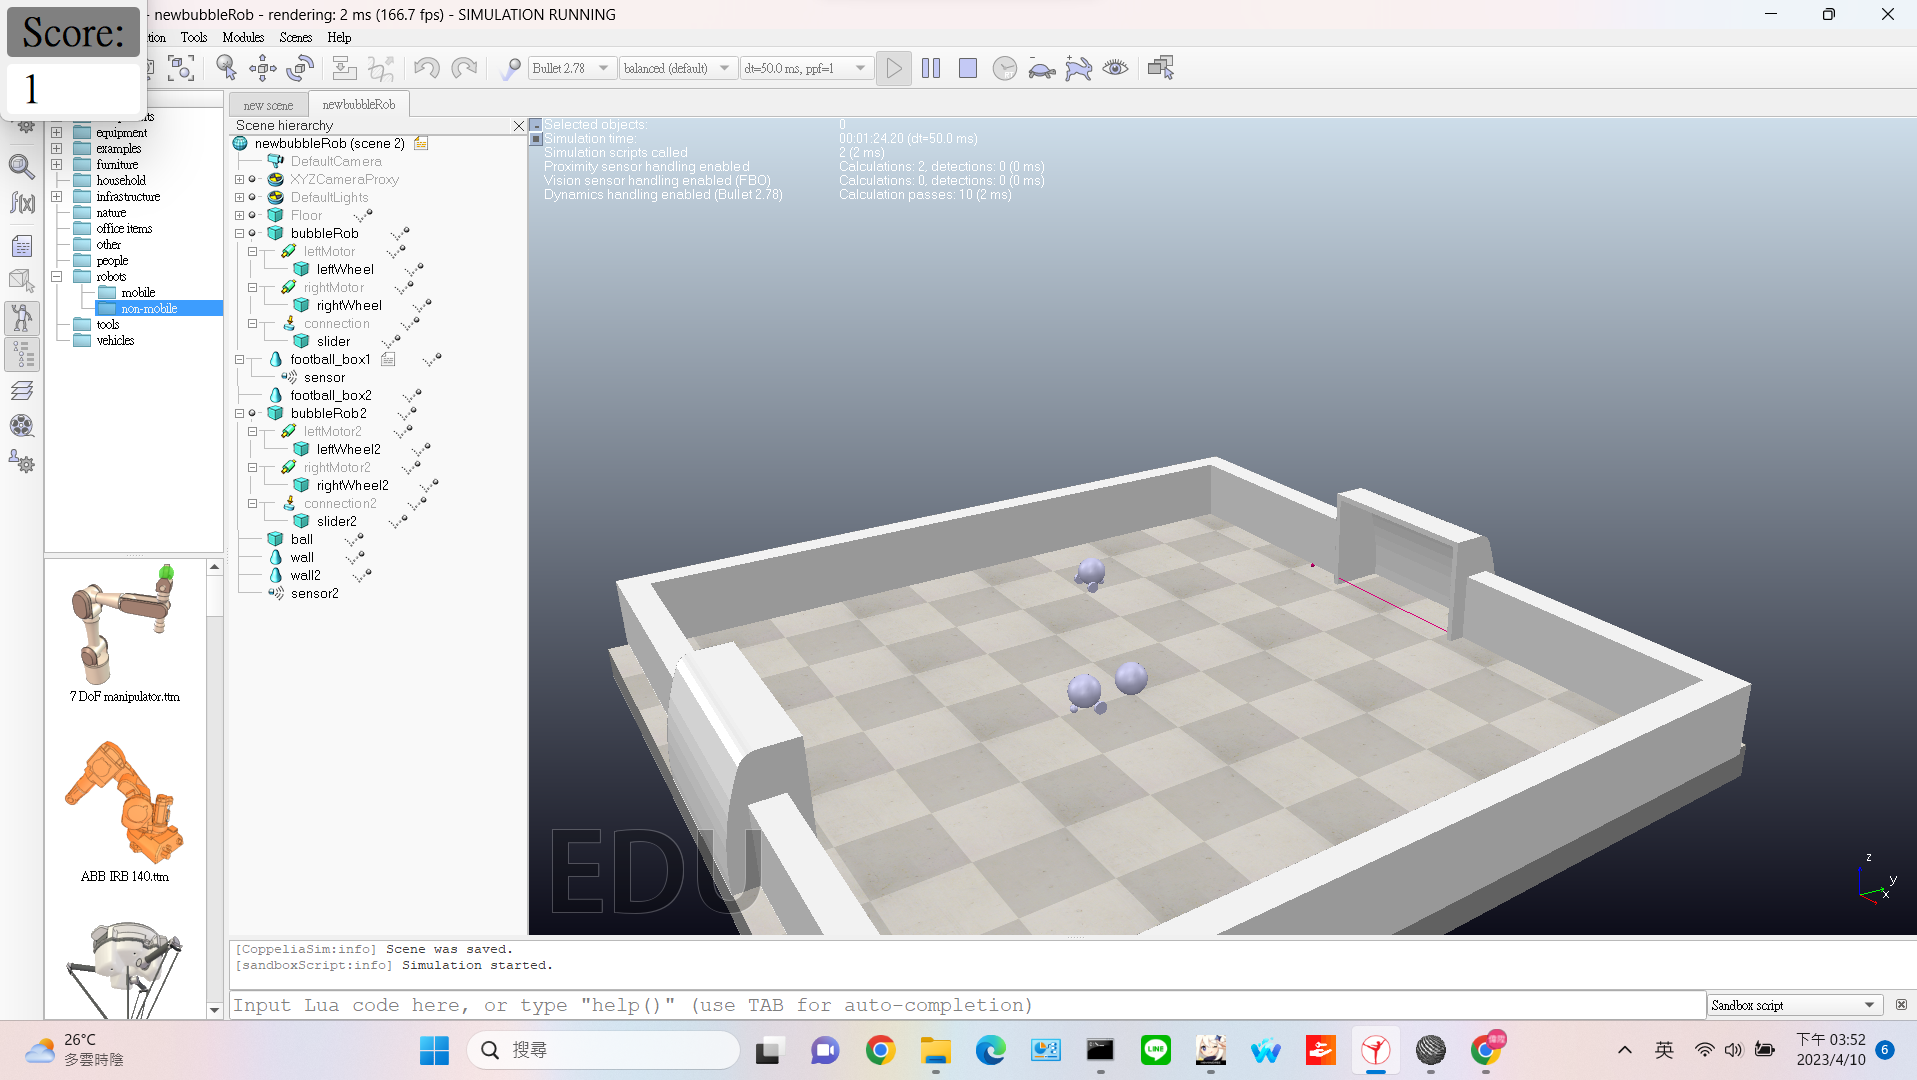
\includegraphics[angle=0,width=15cm]{football}
\end{center}

詳情可見\\
\href{https://mdecd2023.github.io/football-apj1/content/ag2.html}{https://mdecd2023.github.io/football-apj1/content/ag2.html}\\